% Abstract
\begin{center}
	\begin{table}[h!]
		\begin{tabular}{|p{50mm}|p{110mm}|}
			\hline
			\thead{
\includegraphics[width=33mm]{htlhl_bildung_mit_zukunft}} &
			\thead{
				\textbf{HÖHERE TECHNISCHE BUNDESLEHRANSTALT HOLLABRUNN} \\
				\textbf{COLLEGE of ENGINEERING } \\
				\hline \\
				\Large{\textbf{Information Technology}}} \\
			\hline
		\end{tabular}
	\end{table}
	~ \\
	~ \\
	\Huge{\textbf{DIPLOMA THESIS}}\\
	\LARGE{\textbf{Documentation}}
	~ \\
	~ \\
	\begin{table}[h!]
		\begin{tabular}{|p{50mm}|p{110mm}|}
			\hline
			\thead{Author(s)} &
			\thead{\schuelerA, \schuelerB, \\ \schuelerC, \schuelerD} \\
			\hline
			\thead{From \\ Academic year} &
			\thead{\aktuellesSchuljahr} \\
			\hline
			\thead{Topic} &
			\thead{\daTitel} \\
			\hline
			\thead{Co-operation partners} &
			\thead{X-Works} \\
			\hline
		\end{tabular}
	\end{table}
	\begin{table}[h!]
    \centering
    \begin{tabular}{|p{50mm}|p{110mm}|}
        \hline
        \makecell[l]{\small Task Description} &
        \small{This diploma project develops 'EduShelf', a web-based platform for managing educational content. 
        It provides students and teachers with a centralized solution for organizing documents and leveraging AI-powered information retrieval (RAG -- Retrieval Augmented Generation).
        The system integrates a modern web frontend, a backend for data processing and storage, and a dedicated AI server for intelligent chat functionality.} \\
        \hline
    \end{tabular}
\end{table}

\begin{table}[h!]
    \centering
    \begin{tabular}{|p{50mm}|p{110mm}|}
        \hline
        \makecell[l]{\small Implementation} &
        \small{The frontend is built with React for a responsive, user-friendly interface. 
        The .NET backend manages data storage and processing, while a Python/Ollama-based AI server handles LLM operations for the chat. 
        Docker containerization ensures easy deployment and scalability.} \\
        \hline
    \end{tabular}
\end{table}

\begin{table}[h!]
    \centering
    \begin{tabular}{|p{50mm}|p{110mm}|}
        \hline
        \makecell[l]{\small Results} &
        \small{The result is a fully functional 'EduShelf' platform featuring user authentication, document upload and indexing, and an interactive AI chat. 
        Users can manage their document libraries and obtain instant answers from their study materials, demonstrating the effective integration of modern web technologies and AI in education.} \\
        \hline
    \end{tabular}
\end{table}


	\newpage

    \newpage



\iffalse

% Abstract text insertion
\begin{abstract}
    \section*{Kurzfassung (Deutsch)}
    Im Rahmen dieser Diplomarbeit wird die Entwicklung einer innovativen App für Teamkommunikation und Aufgabenmanagement vorgestellt. Ziel ist es, eine nahtlose Lösung bereitzustellen, die Organisationen und Teams dabei unterstützt, effizient zusammenzuarbeiten und Projekte erfolgreich zu managen. Die App integriert essenzielle Funktionen wie Authentifizierung, Kalender, Chat inklusive KI-gestütztem Chatbot sowie die Erstellung und Verwaltung von Teams. Darüber hinaus ermöglicht sie ein umfassendes Budget- und Zeitmanagement auf Projektebene.

    Ein zentraler Bestandteil des Projekts ist die Entwicklung nativer Anwendungen für iOS, Android, Desktop und Web sowie eines leistungsfähigen Backends. Das Backend gewährleistet die Verwaltung aller Frontend-Anforderungen, speichert Daten in einer zentralen Datenbank und verarbeitet Benutzeranfragen effizient. Durch die Integration aller Funktionen in einer benutzerfreundlichen Plattform wird die Fragmentierung bestehender Tools überwunden und eine reibungslose Zusammenarbeit gefördert.

    Das geplante Endprodukt stellt eine umfassende Lösung für modernes Projektmanagement dar, die die Bedürfnisse moderner Teams adressiert und die Effizienz sowie den Erfolg in Organisationen steigert.

    \section*{Abstract (English)}
    This thesis presents the development of an innovative app for team communication and task management. The goal is to provide a seamless solution that helps organizations and teams collaborate efficiently and manage projects successfully. The app integrates essential features such as authentication, a calendar, a chat function with an AI-powered chatbot, and tools for creating and managing teams. Additionally, it enables comprehensive budget and time management at the project level.

    A key component of the project is the development of native applications for iOS, Android, Desktop, and Web, alongside a robust backend. The backend ensures the management of all frontend requirements, stores data in a central database, and efficiently processes user requests. By integrating all functionalities into a user-friendly platform, the solution overcomes the fragmentation of existing tools and promotes seamless collaboration.

    The final product is designed to be a comprehensive solution for modern project management, addressing the needs of contemporary teams and enhancing efficiency and success within organizations.
\end{abstract}
\fi

\newpage

\begin{table}[h!]
    \centering
    \begin{tabular}{|p{50mm}|p{110mm}|}
    \hline
    \makecell[l{{p{50mm}}}]{\small{Typische Grafik, Foto etc. (mit Erläuterung)}} &
    \makecell*[{{p{110mm}}}]{\vspace{6mm} 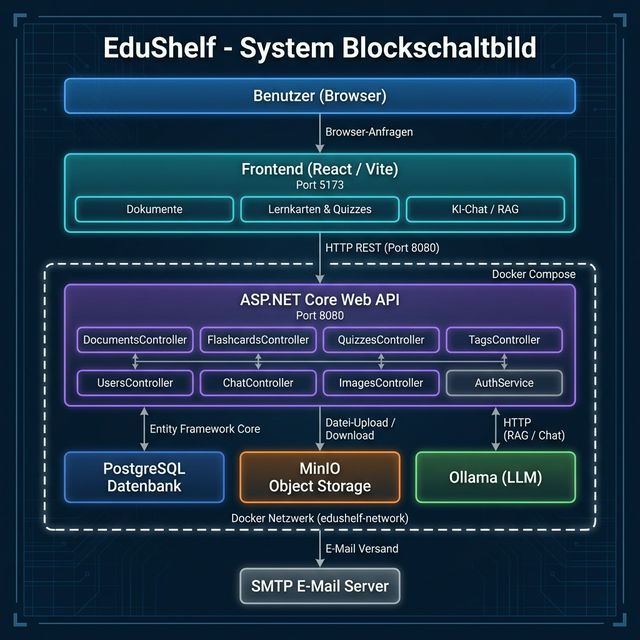
\includegraphics[width=80mm]{img/blockschaltbild.png} \vspace{6mm}} \\ % No file extension here!
    \hline
\end{tabular}
\end{table}
	\begin{table}[h!]
		\begin{tabular}{|p{50mm}|p{110mm}|}
			\hline
			\makecell[l{{p{50mm}}}]{\small{Participation in competitions Awards}} &
			\makecell*[{{p{110mm}}}]{\small{}} \\
			\hline
		\end{tabular}
	\end{table}
	\begin{table}[h!]
		\begin{tabular}{|p{50mm}|p{110mm}|}
			\hline
			\makecell[l{{p{50mm}}}]{
				\small{Accessibility of}\\
				\small{final project thesis}} &
			\makecell*[{{p{110mm}}}]{
				\small{HTL Hollabrunn} \\
				\small{Anton Ehrenfriedstraße 10} \\
				\small{2020 Hollabrunn}} \\
			\hline
		\end{tabular}
	\end{table}
    \vspace{8mm}
	\begin{table}[h!]
		\begin{tabular}{|p{52mm}|p{52mm}|p{52mm}|}
			\hline
			\makecell[l{{p{52mm}}}]{\small{Approval (Date / Signature)} \\ ~ \\ ~ \\} &
			\makecell[l{{p{52mm}}}]{\small{Examiner/s} \\ ~ \\ ~ \\} &
			\makecell[l{{p{52mm}}}]{\small{Head of Department / College} \\ ~ \\ ~ \\} \\
			\hline
		\end{tabular}
	\end{table}
\end{center}

\newpage